\documentclass[14pt]{extbook}
\usepackage{multicol, enumerate, enumitem, hyperref, color, soul, setspace, parskip, fancyhdr} %General Packages
\usepackage{amssymb, amsthm, amsmath, latexsym, units, mathtools} %Math Packages
\everymath{\displaystyle} %All math in Display Style
% Packages with additional options
\usepackage[headsep=0.5cm,headheight=12pt, left=1 in,right= 1 in,top= 1 in,bottom= 1 in]{geometry}
\usepackage[usenames,dvipsnames]{xcolor}
\usepackage{dashrule}  % Package to use the command below to create lines between items
\newcommand{\litem}[1]{\item#1\hspace*{-1cm}\rule{\textwidth}{0.4pt}}
\pagestyle{fancy}
\lhead{Progress Quiz 9}
\chead{}
\rhead{Version B}
\lfoot{9541-5764}
\cfoot{}
\rfoot{Summer C 2021}
\begin{document}

\begin{enumerate}
\litem{
First, find the equation of the line containing the two points below. Then, write the equation in the form $ y=mx+b $ and choose the intervals that contain $m$ and $b$.\[ (10, 9) \text{ and } (2, -4) \]\begin{enumerate}[label=\Alph*.]
\item \( m \in [1.62, 7.62] \hspace*{3mm} b \in [-7.32, -6.9] \)
\item \( m \in [1.62, 7.62] \hspace*{3mm} b \in [-6.14, -5.46] \)
\item \( m \in [1.62, 7.62] \hspace*{3mm} b \in [6.74, 7.29] \)
\item \( m \in [-4.62, -0.62] \hspace*{3mm} b \in [-0.91, 0.3] \)
\item \( m \in [1.62, 7.62] \hspace*{3mm} b \in [-1.54, -0.91] \)

\end{enumerate} }
\litem{
Solve the equation below. Then, choose the interval that contains the solution.\[ -11(15x + 4) = -7(2x + 18) \]\begin{enumerate}[label=\Alph*.]
\item \( x \in [1.1, 1.29] \)
\item \( x \in [-0.99, -0.75] \)
\item \( x \in [-1.81, -1.09] \)
\item \( x \in [0.54, 0.79] \)
\item \( \text{There are no real solutions.} \)

\end{enumerate} }
\litem{
Solve the equation below. Then, choose the interval that contains the solution.\[ -8(-9x -19) = -16(2x + 11) \]\begin{enumerate}[label=\Alph*.]
\item \( x \in [-0.37, 0.13] \)
\item \( x \in [0.17, 0.39] \)
\item \( x \in [0.53, 1.1] \)
\item \( x \in [-3.47, -3.09] \)
\item \( \text{There are no real solutions.} \)

\end{enumerate} }
\litem{
First, find the equation of the line containing the two points below. Then, write the equation in the form $ y=mx+b $ and choose the intervals that contain $m$ and $b$.\[ (7, -3) \text{ and } (-8, -11) \]\begin{enumerate}[label=\Alph*.]
\item \( m \in [-0.94, 0.53] \hspace*{3mm} b \in [-17.27, -11.27] \)
\item \( m \in [0.52, 0.71] \hspace*{3mm} b \in [-13, -8] \)
\item \( m \in [0.52, 0.71] \hspace*{3mm} b \in [-5, 3] \)
\item \( m \in [0.52, 0.71] \hspace*{3mm} b \in [2.73, 8.73] \)
\item \( m \in [0.52, 0.71] \hspace*{3mm} b \in [-7.73, -3.73] \)

\end{enumerate} }
\litem{
Find the equation of the line described below. Write the linear equation in the form $ y=mx+b $ and choose the intervals that contain $m$ and $b$.\[ \text{Parallel to } 4 x + 9 y = 11 \text{ and passing through the point } (-2, -8). \]\begin{enumerate}[label=\Alph*.]
\item \( m \in [-0.68, -0.35] \hspace*{3mm} b \in [8.15, 10.53] \)
\item \( m \in [-2.63, -2.21] \hspace*{3mm} b \in [-9.38, -8.49] \)
\item \( m \in [-0.68, -0.35] \hspace*{3mm} b \in [-6.29, -5.34] \)
\item \( m \in [-0.68, -0.35] \hspace*{3mm} b \in [-9.38, -8.49] \)
\item \( m \in [0.21, 1.07] \hspace*{3mm} b \in [-7.77, -6.24] \)

\end{enumerate} }
\litem{
Write the equation of the line in the graph below in Standard Form $Ax+By=C$. Then, choose the intervals that contain $A, B, \text{ and } C$.
\begin{center}
    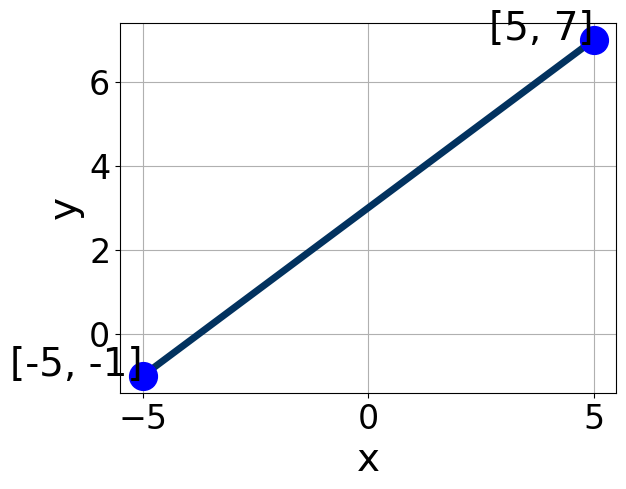
\includegraphics[width=0.5\textwidth]{../Figures/linearGraphToStandardB.png}
\end{center}
\begin{enumerate}[label=\Alph*.]
\item \( A \in [-3.1, 0.9], \hspace{3mm} B \in [-3, -0.4], \text{ and } \hspace{3mm} C \in [-8, -1] \)
\item \( A \in [-7.1, -2.2], \hspace{3mm} B \in [4.9, 6.3], \text{ and } \hspace{3mm} C \in [10, 18] \)
\item \( A \in [0.7, 7.4], \hspace{3mm} B \in [-7.4, -2.9], \text{ and } \hspace{3mm} C \in [-18, -13] \)
\item \( A \in [-3.1, 0.9], \hspace{3mm} B \in [0.1, 2.7], \text{ and } \hspace{3mm} C \in [-1, 4] \)
\item \( A \in [0.7, 7.4], \hspace{3mm} B \in [4.9, 6.3], \text{ and } \hspace{3mm} C \in [10, 18] \)

\end{enumerate} }
\litem{
Solve the linear equation below. Then, choose the interval that contains the solution.\[ \frac{5x + 6}{2} - \frac{7x + 4}{3} = \frac{-4x -4}{7} \]\begin{enumerate}[label=\Alph*.]
\item \( x \in [-7.26, -6.33] \)
\item \( x \in [-3.47, -2.8] \)
\item \( x \in [-1.27, -0.3] \)
\item \( x \in [-8.52, -7.79] \)
\item \( \text{There are no real solutions.} \)

\end{enumerate} }
\litem{
Solve the linear equation below. Then, choose the interval that contains the solution.\[ \frac{-7x + 8}{2} - \frac{-5x -7}{8} = \frac{-6x + 3}{5} \]\begin{enumerate}[label=\Alph*.]
\item \( x \in [-2.9, -0.5] \)
\item \( x \in [6.7, 7.5] \)
\item \( x \in [1.2, 1.8] \)
\item \( x \in [2.4, 3] \)
\item \( \text{There are no real solutions.} \)

\end{enumerate} }
\litem{
Write the equation of the line in the graph below in Standard Form $Ax+By=C$. Then, choose the intervals that contain $A, B, \text{ and } C$.
\begin{center}
    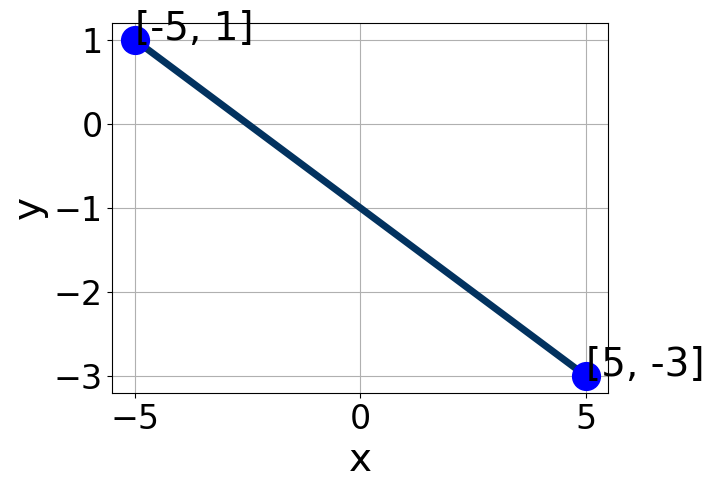
\includegraphics[width=0.5\textwidth]{../Figures/linearGraphToStandardCopyB.png}
\end{center}
\begin{enumerate}[label=\Alph*.]
\item \( A \in [-2.53, -1.94], \hspace{3mm} B \in [-5.7, -3.7], \text{ and } \hspace{3mm} C \in [4.46, 6.57] \)
\item \( A \in [-0.18, 1.68], \hspace{3mm} B \in [-0.5, 2.4], \text{ and } \hspace{3mm} C \in [-2.19, -0.77] \)
\item \( A \in [-0.18, 1.68], \hspace{3mm} B \in [-3.2, -0.3], \text{ and } \hspace{3mm} C \in [0.79, 1.05] \)
\item \( A \in [1.39, 2.92], \hspace{3mm} B \in [-5.7, -3.7], \text{ and } \hspace{3mm} C \in [4.46, 6.57] \)
\item \( A \in [1.39, 2.92], \hspace{3mm} B \in [4.8, 5.4], \text{ and } \hspace{3mm} C \in [-5.32, -3.7] \)

\end{enumerate} }
\litem{
Find the equation of the line described below. Write the linear equation in the form $ y=mx+b $ and choose the intervals that contain $m$ and $b$.\[ \text{Parallel to } 3 x + 7 y = 8 \text{ and passing through the point } (-5, 7). \]\begin{enumerate}[label=\Alph*.]
\item \( m \in [-0.99, 0.22] \hspace*{3mm} b \in [-4.86, -1.86] \)
\item \( m \in [-0.99, 0.22] \hspace*{3mm} b \in [-0.14, 5.86] \)
\item \( m \in [-3.3, -1.72] \hspace*{3mm} b \in [-0.14, 5.86] \)
\item \( m \in [-0.99, 0.22] \hspace*{3mm} b \in [12, 16] \)
\item \( m \in [-0.39, 0.98] \hspace*{3mm} b \in [9.14, 10.14] \)

\end{enumerate} }
\end{enumerate}

\end{document}